64. Возможны два случая расположения точек $P$ и $K$ на стороне $BC.$ В первом случае точки расположены в порядке $B,\ P,\ K,\ C.$
\begin{figure}[ht!]
\center{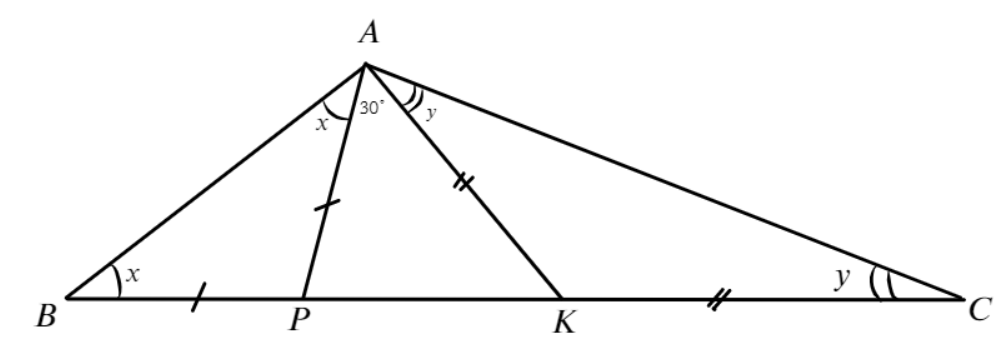
\includegraphics[scale=0.35]{g64-1.png}}
\end{figure}\\
Треугольники $APB$ и $AKC$ являются равнобедренными, обозначим их углы при основании буквами $x$ и $y.$ Тогда из треугольника $ABC$ имеем $2x+2y+30^\circ=180^\circ,\ x+y=75^\circ.$ Таким образом, $\angle BAC=x+y+30^\circ=75^\circ+30^\circ=105^\circ.$\\
Во втором случае точки расположены в порядке $B,\ K,\ P,\ C.$
\begin{figure}[ht!]
\center{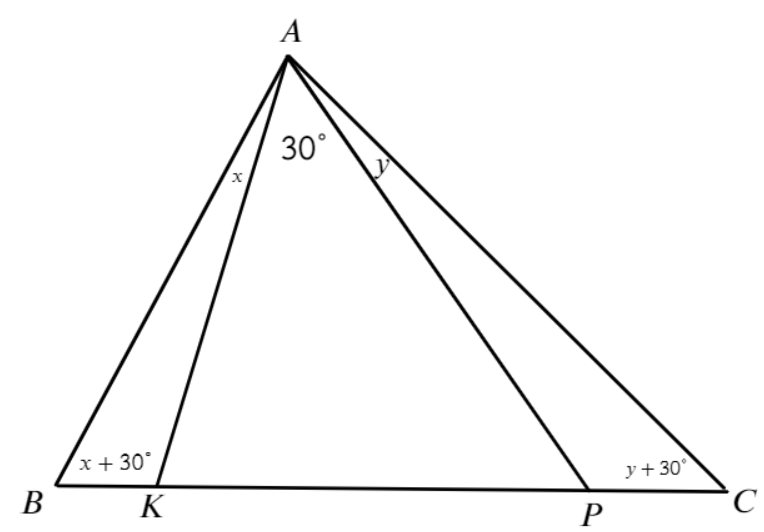
\includegraphics[scale=0.35]{g64-2.png}}
\end{figure}\\
В этом случае обозначим $\angle BAK=x,\ \angle PAC=y,$ тогда $\angle B=x+30^\circ,\ \angle C=y+30^\circ.$ Из треугольника $ABC$ имеем $x+30^\circ+y+30^\circ+x+y+30^\circ=180^\circ,\ x+y=45^\circ.$ Таким образом, $\angle BAC=x+y+30^\circ=45^\circ+30^\circ=75^\circ.$\\
